\documentclass{book}

\usepackage{amssymb}
\usepackage{amsmath}
\usepackage{amsthm}
\usepackage{arydshln}
\usepackage{calc}
\usepackage{cancel}
\usepackage{caption}
\usepackage{cite}
\usepackage{color}
\usepackage{enumitem}
\usepackage{esint}
\usepackage{etoolbox}
\usepackage{float}
\usepackage{framed}
\usepackage{fullpage}
\usepackage{gensymb}
\usepackage[margin=1in]{geometry}
\usepackage{graphicx}
\usepackage{listings}
\usepackage{multirow}
\usepackage{subfiles}
\usepackage{rsfso}
\usepackage{tikz}
\usepackage{tikz-3dplot}
\usepackage{ushort}
\usepackage{wrapfig}
\usepackage{xcolor}
\usepackage{soul}
\usepackage{epstopdf}

% pdf versions
\pdfoptionpdfminorversion=7

% handle page stretching
\raggedbottom

% Graphics file location
\graphicspath{{Graphics/}{../Graphics/}}

% Use for drawings
\usetikzlibrary{angles,arrows,calc,decorations,intersections,patterns,positioning,quotes}
\newcommand{\midarrow}{\tikz \draw[-latex] (0,0) -- +(.1,0);}

% Tikz commands for drawing block diagrams, etc...
\tikzset{%
	block/.style    = {draw, rectangle, minimum height = 2em, minimum width = 2em},
	sum/.style      = {draw, circle}, % Adder
	input/.style    = {fill=white, rectangle}, % Input
	output/.style   = {fill=white, rectangle}, % Output
	waypoint/.style   = {coordinate}, % Output
}

\tikzset{
	saveuse path/.code 2 args={
		\pgfkeysalso{#1/.style={insert path={#2}}}%
		\global\expandafter\let\csname pgfk@\pgfkeyscurrentpath/.@cmd\expandafter\endcsname
		% not optimal as it is now global through out the document
		\csname pgfk@\pgfkeyscurrentpath/.@cmd\endcsname
		\pgfkeysalso{#1}},
	/pgf/math set seed/.code=\pgfmathsetseed{#1}}

% Define Laplace, Fourier transform symbols
\newcommand{\LT}{\mathcal{L}}
\newcommand{\FT}{\mathcal{F}}

% Define adjugate function
\newcommand{\adj}{\text{adj}}

% Define rank function
\newcommand{\rank}{\text{rank}}

% commands to speed up writing j\omega and s-plane
\newcommand{\jw}{j\omega}
\newcommand{\spl}{s\textrm{-plane}}
% Clean up overline/underline for math mode
\def\obar#1{\bar{#1}}
\def\ubar#1{\ushort{#1}}

\newcommand{\exmp}{\subsubsection*{Example}}
\newcommand{\nib}{\noindent$ \bullet\ $}


\begin{document}
	\chapter*{Lecture 11}
	Last lecture: Complete seven rules for drawing a root locus.
	
	\noindent Today: Continue discussion of root locus\\
	\nib Closed-loop zeros\\
	\nib Control system design via root locus

\section*{Angle and Magnitude Criterion}
We will begin with an example of applying the angle and magnitude criteria. Recall,
\begin{equation}
\textbf{Angle Criterion:}\quad \sum^{m}\theta_{zi}-\sum^{n}\theta_{pi} = 180^\circ \pm \ell 360^\circ, \quad \ell = 0,1,2,\ldots
\end{equation}
The angle criterion tells us if a point is on the root locus.
\begin{equation}
\textbf{Magnitude Criterion:}\quad \frac{\prod^{n}M_{pi}}{\prod^{m}M_{zi}} = K
\end{equation}
\begin{center}
	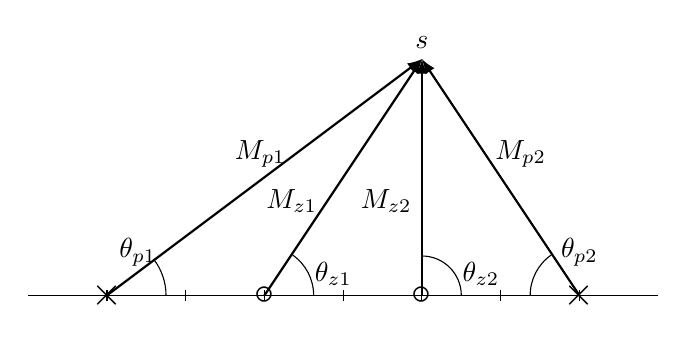
\begin{tikzpicture}[scale = 1]
	\draw (-7,0) -- (1,0);
	\foreach \x in {-6,-5,-4,-3,-2,-1,0}
	\draw (\x cm,2pt) -- (\x cm,-2pt);
	\node at (-6,0) {\Large$ \times $};
	\draw[thick,-latex] (-6,0) -- node[left,pos=0.6] {$ M_{p1} $} (-2,3) node[above] {$ s $};
	\draw (-5.25,0) arc (0:38:0.75);
	\node[above left] at (-5.25,0.25) {$ \theta_{p1} $};
	\node at (0,0) {\Large$ \times $};
	\draw[thick,-latex] (0,0) -- node[right,pos=0.6] {$ M_{p2} $} (-2,3);
	\draw (-0.625,0) arc (180:125:0.625);
	\node[above] at (0,0.25) {$ \theta_{p2} $};
	\node at (-4,0) {\Large$ \circ $};
	\draw[thick,-latex] (-4,0) -- node[left,pos=0.4] {$ M_{z1} $} (-2,3);
	\draw (-3.375,0) arc (0:55:0.625);
	\node[above] at (-3.125,0) {$ \theta_{z1} $};
	\node at (-2,0) {\Large$ \circ $};
	\draw[thick,-latex] (-2,0) -- node[left,pos=0.4] {$ M_{z2} $} (-2,3);
	\draw (-1.5,0) arc (0:90:0.5);
	\node[above] at (-1.25,0) {$ \theta_{z2} $};
	\end{tikzpicture}
\end{center}

\exmp
Consider the following system:
\begin{center}
	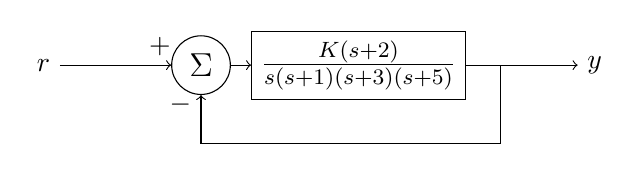
\begin{tikzpicture}[node distance = 2cm]
	\node[input] (r) at (0,0) {$ r $};
	\node[sum,right of=r] (sum) {\large$ \Sigma $};
	\node[block, right of=sum] (tf) {\large$ \frac{K(s+2)}{s(s+1)(s+3)(s+5)} $};
	\node[waypoint,below of=tf,node distance = 1cm] (wp) {};
	\node[output, right of=tf,node distance = 3cm] (y) {$ y $};
	\draw[->] (r) -- node[above,pos=0.9] {$ + $} (sum);
	\draw[->] (sum) -- (tf);
	\draw[->] (tf) -- (y);
	\draw[->] ($(tf)!0.6!(y)$) |- (wp) -| node[left,pos=0.9] {$ - $} (sum);
	\end{tikzpicture}
\end{center}
Then,
\[ \sigma = \frac{0+(-1)+(-3)+(-5) - (-2)}{4-1}=-\frac{7}{3} \]
\[ \theta = \frac{180^\circ+\ell 360^\circ}{3-0} = 60^\circ + \ell120^\circ,\ \ell = 0, 1, 2 \quad\Rightarrow\quad \theta= 60^\circ,180^\circ,300^\circ \]
At what gain does the system go unstable (the locus crosses into the right-hand plane)? 
\begin{center}
	\begin{tikzpicture}[xscale=1,yscale=0.6]
	\draw (-7,0) -- (2,0);
	\draw (0,-5) -- (0,5);
	\foreach \x in {-6,-5,-4,-3,-2,-1,0,1} \draw (\x cm,2pt) -- (\x cm,-2pt);
	\foreach \x in {-4,-3,-2,-1,0,1,2,3,4} \draw (2pt,\x cm) -- (-2pt,\x cm);
	\node at (0,0) {\Large$ \times $};
	\node at (-1,0) {\Large$ \times $};
	\node at (-3,0) {\Large$ \times $};
	\node at (-5,0) {\Large$ \times $};
	\node at (-2,0) {\Large$ \circ $};
	\draw[thick] (-1,0.01) -- (0,0.01);
	\draw[thick,-latex] (-3,0.01) -- (-2,0.01);
	\draw[thick,-latex] (-5,0.01) -- (-7,0.01);
	\draw[thick] (-0.5,0) arc (180:150:8);
	\draw[thick] (-0.5,0) arc (180:210:8);
	\draw[dashed] (0,-4.041) -- (-2.3333,0) -- (0,4.041);
	\draw[dotted,thick] (-5,0) -- (0,2.8) -- (-3,0);
	\draw[dotted,thick] (-2,0) -- (0,2.8) -- (-1,0);
	\end{tikzpicture}
\end{center}
This occurs at approximate $ s\approx \pm2.8j $. Therefore,
\[ K = \frac{\prod M_{pi}}{\prod M_{zi}} = \frac{(5.6)(4.1)(3.0)(2.8)}{3.5} = 55.1 \]
We can confirm this in Matlab and find $ K=60.1 $. So, our hand computation is fairly accurate.

\noindent At what gain does the locus break away from the real axis? First, we compute the break away point:
\[ \sum^m \frac{1}{\sigma_b+z_i} = \sum^n \frac{1}{\sigma_b+p_i} \]
\[ \frac{1}{\sigma_b}+\frac{1}{\sigma_b+1}+\frac{1}{\sigma_b+3}+\frac{1}{\sigma_b+5} = \frac{1}{\sigma_b+2} \]
So, the breakaway is at $ \sigma_b \approx -0.5 $. Then,
\[ K = \frac{\prod M_{pi}}{\prod M_{zi}} = \frac{(4.5)(2.5)(0.5)(0.5)}{1.5} = 1.88 \]

\noindent Is a second-order approximation valid for this system?
\begin{itemize} 
	\item The relative dominance of closed-loop poles is determined by the ratio of the real parts of the closed-loop poles as well as by the relative magnitudes of the residues evaluated at the closed-loop poles. The magnitude of the residues depend on both closed-loop poles and zeros.
	\item If the ratios of the real parts of the closed-loop poles exceed 5 and there are no zeros nearby, then the closed-loop poles nearest the $j\omega$-axis dominate the transient response behavior. 
	\item Those closed-loop poles that have dominant effects on the transient response behavior are called \textit{dominant closed loop poles}.
  
\end{itemize}
Need to always be careful about approximating higher order systems with its second order counterparts. We want the 2nd-order pair to be 5 times slower than the other poles. \\
\begin{center}
	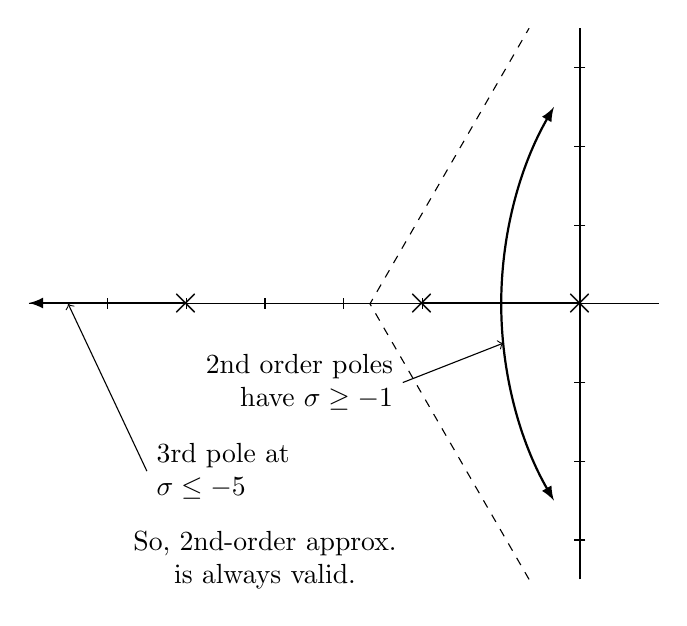
\begin{tikzpicture}[scale=1]
	\draw (-7,0) -- (1,0);
	\draw (0,-3.5) -- (0,3.5);
	\foreach \x in {-6,-5,-4,-3,-2,-1} \draw (\x cm,2pt) -- (\x cm,-2pt);
	\foreach \x in {-3,-2,-1,0,1,2,3} \draw (2pt,\x cm) -- (-2pt,\x cm);
	\node at (0,0) {\Large$ \times $};
	\node at (-2,0) {\Large$ \times $};
	\node at (-5,0) {\Large$ \times $};
	\draw[thick] (0,0.01) -- (-2,0.01);
	\draw[thick,-latex] (-5,0.01) -- (-7,0.01);
	\draw[thick,-latex] (-1,0) arc (180:150:5);
	\draw[thick,-latex] (-1,0) arc (180:210:5);
	\draw[dashed] (-0.646,-3.5) -- (-2.6667,0) -- (-0.646,3.5);
	
	% \draw (-2,-2) node[left] {pole at $ s=\sigma+\jw $} -- (-0.95,1);
	\draw[->] (-2.25,-1) node[left,align=right] {2nd order poles\\have $ \sigma\geq-1 $} -- (-0.975,-0.5);
	\draw[->] (-5.5,-2.125) node[right,align=left] {3rd pole at\\$ \sigma\leq-5 $} -- (-6.5,0);
	
	\node[align=center] at (-4,-3.25) {So, 2nd-order approx.\\is always valid.};
	\end{tikzpicture}
\end{center}
\begin{center}
	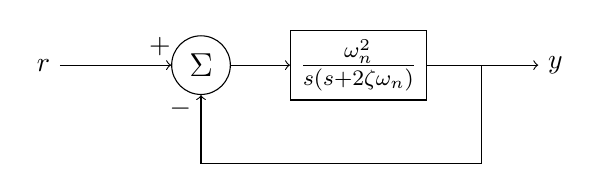
\begin{tikzpicture}[node distance = 2cm]
	\node[input] (r) at (0,0) {$ r $};
	\node[sum,right of=r] (sum) {\large$ \Sigma $};
	\node[block, right of=sum] (g) {\large$ \frac{\omega_n^2}{s(s+2\zeta\omega_n)} $};
	\node[waypoint,below of=g,node distance = 1.25cm] (h) {};
	\node[output, right of=g,node distance = 2.5cm] (y) {$ y $};
	\draw[->] (r) -- node[above,pos=0.9] {$ + $} (sum);
	\draw[->] (sum) -- (g);
	\draw[->] (g) -- (y);
	\draw[->] ($(g)!0.625!(y)$) |- (h) -| node[left,pos=0.9] {$ - $} (sum);
	\end{tikzpicture}
\end{center}
A second order closed-loop transfer function comes from the following open-loop transfer function:
\[ \frac{\hat{y}}{\hat{r}} = \frac{\frac{\omega_n^2}{s(s+2\zeta\omega_n)}}{1+\frac{\omega_n^2}{s(s+2\zeta\omega_n)}} = \frac{\omega_n^2}{s^2+2\zeta\omega_ns + \omega_n^2} \]
For instance, poles at $ s=-1\pm2j $ give:
\[ \frac{\hat{y}}{\hat{r}} = \frac{5}{s^2+2s+5} \]

\section*{Closed-Loop Zeros}
Does the root locus tell us about the closed-loop zeros? Consider this system:
\begin{center}
	\begin{tikzpicture}[scale=0.75]
	\draw (-10,0) -- (2,0);
	\draw (0,-1.5) -- (0,1.5);
	\foreach \x in {-9,-8,-7,-6,-5,-4,-3,-2,-1,0,1} \draw (\x cm,2pt) -- (\x cm,-2pt);
	\node at (-8,0) {\Large$ \times $};
	\node at (-6,0) {\Large$ \circ $};
	\node at (-4,0) {\Large$ \times $};
	\node at (-2,0) {\Large$ \circ $};
	\node at (0,0) {\Large$ \times $};
	\node[below] at (-8,-0.05) {$ -8 $};
	\node[below] at (-6,-0.05) {$ -6 $};
	\node[below] at (-4,-0.05) {$ -4 $};
	\node[below] at (-2,-0.05) {$ -2 $};
	\node[below right] at (0,-0.05) {$ 0 $};
	\draw[thick,-latex] (-8,0) -- (-10,0);
	\draw[thick,-latex] (-4,0) -- (-6,0);
	\draw[thick,-latex] (0,0) -- (-2,0);
	\end{tikzpicture}
\end{center}

\begin{center}
	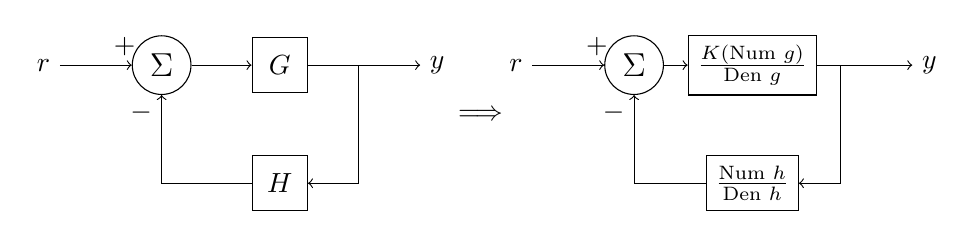
\begin{tikzpicture}[node distance = 1.5cm]
	\node[input] (r) at (0,0) {$ r $};
	\node[sum,right of=r] (sum) {\large$ \Sigma $};
	\node[block, right of=sum] (g) {$ G $};
	\node[block,below of=g] (h) {$ H $};
	\node[output, right of=g,node distance = 2cm] (y) {$ y $};
	\draw[->] (r) -- node[above,pos=0.9] {$ + $} (sum);
	\draw[->] (sum) -- (g);
	\draw[->] (g) -- (y);
	\draw[->] ($(g)!0.5!(y)$) |- (h);
	\draw[->] (h) -| node[left,pos=0.9] {$ - $} (sum);
	
	\node[input] (r2) at (6,0) {$ r $};
	\node[sum,right of=r2] (sum2) {\large$ \Sigma $};
	\node[block, right of=sum2] (g2) {$ \frac{K(\text{Num }g)}{\text{Den }g} $};
	\node[block,below of=g2] (h2) {$ \frac{\text{Num }h}{\text{Den }h} $};
	\node[output, right of=g2,node distance = 2.25cm] (y2) {$ y $};
	\draw[->] (r2) -- node[above,pos=0.9] {$ + $} (sum2);
	\draw[->] (sum2) -- (g2);
	\draw[->] (g2) -- (y2);
	\draw[->] ($(g2)!0.5!(y2)$) |- (h2);
	\draw[->] (h2) -| node[left,pos=0.9] {$ - $} (sum2);
	
	\node at ($(g)!0.425!(h2)$) {$ \Longrightarrow $};
	\end{tikzpicture}
\end{center}
We will solve for the closed-loop transfer function. What are the closed-loop zeros?

\[ CLTF = \frac{\hat{y}}{\hat{r}} = \frac{\frac{K(\text{Num }g)}{\text{Den }g}}{1+\frac{K(\text{Num }g)}{\text{Den }g}\cdot\frac{\text{Num }h}{\text{Den }h}} = \frac{K\cdot\text{Num }g\cdot \text{Den }h}{\text{Den }g\cdot\text{Den }h+K\cdot\text{Num }g\cdot\text{Num }h} \]

So, the closed loop zeros satisfy:
\[ K\cdot\text{Num }g\cdot \text{Den }h = 0 \]
\[ \text{Num }g\cdot \text{Den }h = 0 \]
Therefore:
\begin{itemize}
	\item The closed-loop zeros are the zeros of the forward path and the poles of the return path.
	\item The closed-loop zeros don't migrate with $ K $.
	\item The closed-loop zeros are clearly not shown on the root locus.
\end{itemize}

For instance, these systems have the same root locus but different closed-loop zeros:
\begin{center}
	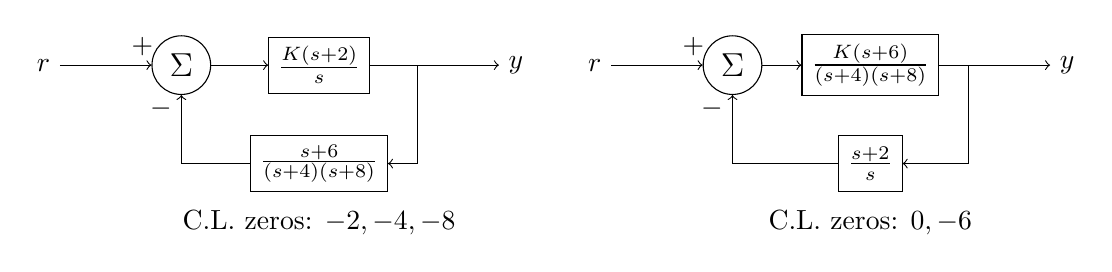
\begin{tikzpicture}[node distance = 1.75cm]
	\node[input] (r) at (0,0) {$ r $};
	\node[sum,right of=r] (sum) {\large$ \Sigma $};
	\node[block, right of=sum] (g) {$ \frac{K(s+2)}{s} $};
	\node[block,below of=g,node distance = 1.25cm] (h) {$ \frac{s+6}{(s+4)(s+8)} $};
	\node[output, right of=g,node distance = 2.5cm] (y) {$ y $};
	\draw[->] (r) -- node[above,pos=0.9] {$ + $} (sum);
	\draw[->] (sum) -- (g);
	\draw[->] (g) -- (y);
	\draw[->] ($(g)!0.5!(y)$) |- (h);
	\draw[->] (h) -| node[left,pos=0.9] {$ - $} (sum);
	\node[below of=g,node distance = 2cm] {C.L. zeros: $ -2,-4,-8 $};
	
	\node[input] (r2) at (7,0) {$ r $};
	\node[sum,right of=r2] (sum2) {\large$ \Sigma $};
	\node[block, right of=sum2] (g2) {$ \frac{K(s+6)}{(s+4)(s+8)} $};
	\node[block,below of=g2,node distance = 1.25cm] (h2) {$ \frac{s+2}{s} $};
	\node[output, right of=g2,node distance = 2.5cm] (y2) {$ y $};
	\draw[->] (r2) -- node[above,pos=0.9] {$ + $} (sum2);
	\draw[->] (sum2) -- (g2);
	\draw[->] (g2) -- (y2);
	\draw[->] ($(g2)!0.5!(y2)$) |- (h2);
	\draw[->] (h2) -| node[left,pos=0.9] {$ - $} (sum2);
	\node[below of=g2,node distance = 2cm] {C.L. zeros: $ 0,-6 $};
	\end{tikzpicture}
\end{center}

\section*{Control system design via root locus}
Consider the system shown:
\begin{center}
	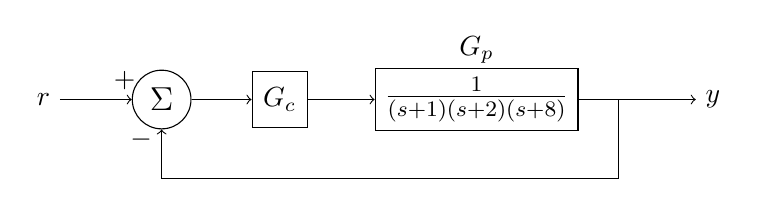
\begin{tikzpicture}[node distance = 1.5cm]
	\node[input] (r) at (0,0) {$ r $};
	\node[sum,right of=r] (sum) {\large$ \Sigma $};
	\node[block, right of=sum] (gc) {$ G_c $};
	\node[block, right of=gc,node distance = 2.5cm] (gp) {\large$ \frac{1}{(s+1)(s+2)(s+8)}$};
	\node[waypoint,below of=gp,node distance = 1cm] (wp) {};
	\node[output, right of=gp,node distance = 3cm] (y) {$ y $};
	\draw[->] (r) -- node[above,pos=0.9] {$ + $} (sum);
	\draw[->] (sum) -- (gc);
	\draw[->] (gc) -- (gp);
	\draw[->] (gp) -- (y);
	\draw[->] ($(gp)!0.6!(y)$) |- (wp) -| node[left,pos=0.9] {$ - $} (sum);
	\node[above of = gp, node distance = 0.625cm] {$ G_p $};
	\end{tikzpicture}
\end{center}
Find $ G_c $ so that a unit step input at $ r(t) $ leads to a $ y(t) $ response that meets the following requirements:
\begin{enumerate}
	\item overshoot $ \leq 20\% $
	\item peak time $ \leq 2 $ seconds
	\item steady-state error $ \leq $ 0.4
	\item system must remain stable
\end{enumerate}

Let's start by trying a proportional controller $ G_c = K_p $ and sketching a root locus. Proceeding through the first 4 rules, we have:
\begin{center}
	\begin{tikzpicture}[scale=.75]
	\draw (-10,0) -- (2,0);
	\draw (0,-2) -- (0,2);
	\foreach \x in {-9,-8,-7,-6,-5,-4,-3,-2,-1,0,1} \draw (\x cm,2pt) -- (\x cm,-2pt);
	\node at (-1,0) {\Large$ \times $};
	\node at (-2,0) {\Large$ \times $};
	\node at (-8,0) {\Large$ \times $};
	\draw[thick] (-1,0.01) -- (-2,0.01);
	\draw[thick] (-8,0.01) -- (-10,0.01);
%	\draw[thick] (-1.5,0) arc (180:150:3);
%	\draw[thick] (-1.5,0) arc (180:210:3);
%	\draw[dashed] (-0.845,-2) -- (-2,0) -- (-0.845,2);
	\end{tikzpicture}
\end{center}
Next, we compute the asymptote center and angles.
\[ \sigma = \frac{-1+(-2)+(-8)}{3-0}=-\frac{11}{3} \]
\[ \theta = \frac{180^\circ+\ell 360^\circ}{3-0} = 60^\circ + \ell120^\circ,\ \ell = 0, 1, 2 \quad\Rightarrow\quad \theta= 60^\circ,180^\circ,300^\circ \]
So, we can sketch the following root locus: \textit{(next page)}

\begin{itemize}
	\item For this system, we will have two poles near the imaginary axis and one pole much further left. 
	\begin{itemize}
		\item We might be able to treat this as a 2nd-order system
	\end{itemize}
	\item No closed-loop zeros
	\item Let's review what we know about 2nd order systems without zeros.
\end{itemize} 

From Lecture 6:
\begin{center}
	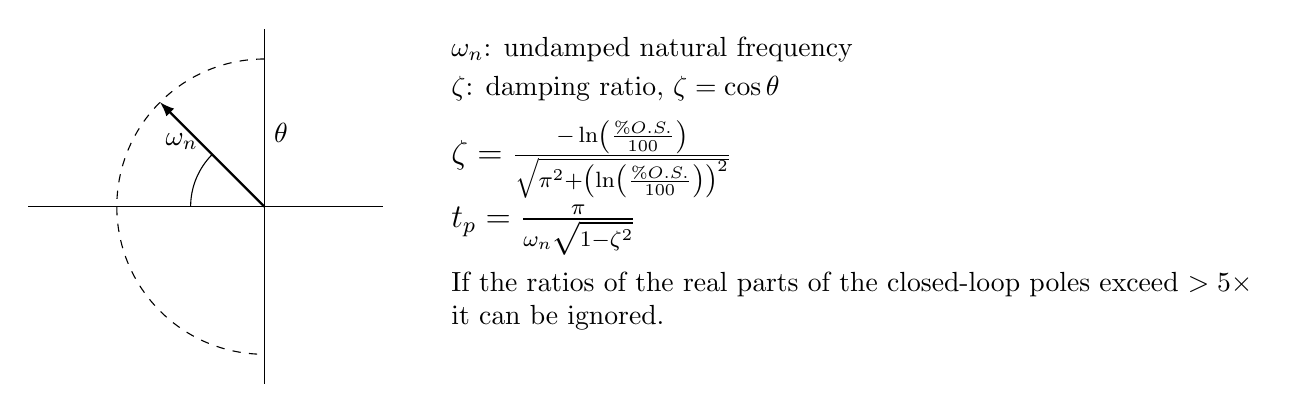
\begin{tikzpicture}[scale=1.5]
		\draw (-2,0) -- (1,0);
		\draw (0,-1.5) -- (0,1.5);
		\draw[dashed] (0,1.25) arc (90:270:1.25);
		\draw[thick,-latex] (0,0) -- (-0.884,0.884);
		\draw (-0.625,0) arc (180:135:0.625);
		\node[right] at (0,.625) {$ \theta $};
		\node[below] at (-0.7,0.7) {$ \omega_n $};
		\node[right] at (1.5, 1.333) {$ \omega_n $: undamped natural frequency};
		\node[right] at (1.5, 1) {$ \zeta $: damping ratio, $ \zeta =\cos\theta$};
		
		\node[right] at (1.5, 0.4) {\large$ \zeta = \frac{-\ln\left(\frac{ \%O.S.}{100}\right)}{\sqrt{\pi^2+\left(\ln\left(\frac{ \%O.S.}{100}\right)\right)^2}} $};
		
		\node[right] at (1.5, -0.2) {\large$ t_p = \frac{\pi}{\omega_n\sqrt{1-\zeta^2}} $};
		
		\node[right, align=left] at (1.5,-0.8) {If the ratios of the real parts of the closed-loop poles exceed $ >5\times $ \\ it can be ignored.};
	\end{tikzpicture}
\end{center}

\begin{center}
	\begin{tikzpicture}[scale=.4]
		\draw (-10,0) -- (2,0);
		\draw (0,-7) -- (0,7);
		\foreach \x in {-9,-8,-7,-6,-5,-4,-3,-2,-1,0,1} \draw (\x cm,2pt) -- (\x cm,-2pt);
		\foreach \x in {-6,-5,-4,-3,-2,-1,0,1,2,3,4,5,6} \draw (2pt,\x cm) -- (-2pt,\x cm);
		\node at (-1,0) {\Large$ \times $};
		\node at (-2,0) {\Large$ \times $};
		\node at (-8,0) {\Large$ \times $};
		\draw[thick] (-1,0.01) -- (-2,0.01);
		\draw[thick] (-8,0.01) -- (-10,0.01);
		\draw[thick] (-1.5,0) arc (180:150:11.5);
		\draw[thick] (-1.5,0) arc (180:210:11.5);
		\draw[dashed] (0,-6.351) -- (-3.6667,0) -- (0,6.351);
	\end{tikzpicture}
\end{center}

We can compute the damping ratio and natural frequency requirements for this system. 
\[ \zeta = \frac{-\ln(0.2)}{\sqrt{\pi^2+(\ln 0.2)^2}} \approx 0.46,\quad \theta = \cos^{-1}\zeta = 63^\circ \]
\[ 2 = \frac{\pi}{\omega_n\sqrt{1-0.46^2}} \quad\Rightarrow\quad \omega_n = 1.76 \]
We can plot the circle corresponding to $ \omega_n=1.76 $ and line corresponding to $ \zeta=0.46 $, identify where these intersect the root locus, and then use the Magnitude Criterion to find the associated gain.

\begin{center}
	\begin{tikzpicture}[scale=.75]
	\draw (-10,0) -- (2,0);
	\draw (0,-7) -- (0,7);
	\foreach \x in {-9,-8,-7,-6,-5,-4,-3,-2,-1,0,1} \draw (\x cm,2pt) -- (\x cm,-2pt);
	\foreach \x in {-6,-5,-4,-3,-2,-1,0,1,2,3,4,5,6} \draw (2pt,\x cm) -- (-2pt,\x cm);
	\node at (-1,0) {\Large$ \times $};
	\node at (-2,0) {\Large$ \times $};
	\node at (-8,0) {\Large$ \times $};
	\draw[thick] (-1,0.01) -- (-2,0.01);
	\draw[thick] (-8,0.01) -- (-10,0.01);
	\draw[thick] (-1.5,0) arc (180:147:9.25);
	\draw[thick] (-1.5,0) arc (180:213:9.25);
	\draw[dashed] (0,-6.351) -- (-3.6667,0) -- (0,6.351);
	\draw[dotted,thick] (0,1.76) arc (90:270:1.76);
	\draw[dotted,thick] (0,0) -- (-3,5.434);
	\draw[fill=black] (-1.25,2.25) circle (0.1);
	\draw[fill=black] (-1.45,1) circle (0.1);
	\node[left] at (-1.45,1) {$ K_1 $};
	\node[right] at (-1.25,2.25) {$ K_2 $};
	\node[right] at (0,1.76) {$ \omega_n=1.76 $};
	\node[left] at (-3,5.434) {$ \zeta=0.46 $};
	
%	\node[right] at (-8, -3) {$ K_1\approx at (-1.4,1) $};
%	\node[right] at (-8, -3.6) {$ K_1\approx(6.7)(1.1)(1.2) = 9 $};
%	\node[right] at (-8, -4.7) {$ K_2\approx at (-1.2,2.1) $};
%	\node[right] at (-8, -5.3) {$ K_2\approx (7.1)(2.1)(2.3) = 35 $};
%	\node[right] at (-8, -6.5) {$ \therefore 9 \leq K \leq 35 $};
	
	\draw (-1,0) node[above right] {$ \theta $} arc (180:117.4:1);
	\end{tikzpicture}
\end{center}

Next, let's compute the breakaway point:
\begin{align*}
0 &= \frac{1}{\sigma_b+1} + \frac{1}{\sigma_b+2} + \frac{1}{\sigma_b+8}\\
0 &= 1 + \frac{\sigma_b+1}{\sigma_b+2} + \frac{\sigma_b+1}{\sigma_b+8}\\
0 &= (\sigma_b+2) + (\sigma_b+1) + \frac{(\sigma_b+1)(\sigma_b+2)}{\sigma_b+8}\\
0 &= (\sigma_b+2)(\sigma_b+8) + (\sigma_b+1)(\sigma_b+8) + (\sigma_b+1)(\sigma_b+2)\\
0 &= (\sigma_b^2+10s+16) + (\sigma_b^2+9s+8) + (\sigma_b^2+3s+2)\\
0 &= 3\sigma_b^2+22\sigma_b+26\\
\sigma_b &= -1.48,\ -5.85
\end{align*}
From Rule 4, we know that only $ \sigma_b = -1.48 $ is valid --- the root locus is not on the real axis at $ s=-5.85 $. We are now going to show two methods of graphically computing a gain for this controller.

\paragraph{Method 1:} Graphically approximate the location for $ K_1 $ and $ K_2 $ (e.g., use a ruler).

$s_1 \quad at \quad K_1 \approx at (-1.4,1),$
$K_1 \approx (6.7)\cdot(1.1)\cdot(1.2) = 9$

$s_2 \quad at \quad K_2 \approx at (-1.16, 2.12),$
$K_2 \approx (7.2)\cdot(2.1)\cdot(2.3) = 35$

$\therefore 9 \leq K_p \leq 35$

\paragraph{Method 2:}  Graphically estimate the real value for $ K_1 $ and $ K_2 $, and use geometry to find the imaginary value. For $ K_1 $, we note that the root locus is mostly vertical near the real axis. We can use assume the locus has the same real value as the breakaway point. So, assuming $ K_1 $ is at the point $ (-1.48,\omega_1) $, then
\[ 1.76^2 = 1.48^2 + \omega_1^2 \quad\Rightarrow\quad \omega_1 = \sqrt{1.76^2-1.48^2} = 0.95 \]
The point for $ K_2 $ is slightly right of the breakaway. Estimating $ K_2 $ is at the point $ (-1.2,\omega_2) $, then
\[ \zeta = \cos\theta \quad\Rightarrow\quad \theta = 62.6^\circ \]
\[ \tan\theta = \frac{opp}{adj} \quad\Rightarrow\quad \omega_2 = 1.2\tan(62.6^\circ) = 2.315 \]
Having an estimate of the location of $ K_1 $ and $ K_2 $, we can find the magnitude of each vector to from the open-loop poles to those points. Then, using the Magnitude Criterion,
\begin{align*}
K_1 & \approx |(1.48+0.95j)-1|\cdot|(1.48+0.95j)-2|\cdot|(1.48+0.95j)-8|\\
&\approx \sqrt{0.48^2+0.95^2} \cdot \sqrt{0.52^2+0.95^2} \cdot \sqrt{6.52^2+0.95^2}\\
&\approx (1.064)(1.083)(6.588)\\
&\approx 7.6
\end{align*}
\begin{align*}
K_2 & \approx |(1.2+2.315j)-1|\cdot|(1.2+2.315j)-2|\cdot|(1.2+2.315j)-8|\\
&\approx \sqrt{0.2^2+2.315^2} \cdot \sqrt{0.8^2+2.315^2} \cdot \sqrt{6.8^2+2.315^2}\\
&\approx (2.32)(2.45)(7.18)\\
&\approx 40.8
\end{align*}
So, $ 7.6 \leq K_p \leq 40.8 $.
% This does not seem to be as accurate as graphical approximation. The true point of the root locus at $ \zeta=0.46 $ is about (-1.13,2.2) so assuming the real part is still at -1.5 adds a decent amount of error.

Next, we must check the steady-state error.
\begin{itemize}
	\item Unity feedback
	\item Type 0 system
	\item Stable
\end{itemize}
For a step input:
\[ e_{ss} = \frac{1}{1+\lim_{s\to 0}G_cG_p} \]
\[ e_{ss} = \frac{1}{1+\lim_{s\to 0}\frac{K_p}{(s+1)(s+2)(s+8)}} = \frac{1}{1+\frac{K_p}{16}} = \frac{16}{16+K_p} \]
Alternatively, we can compute the steady-state error directly instead of using system types:
\[ E(s) = \frac{1}{1+G_cG_p}R(s) = \frac{1}{1+\frac{K_p}{(s+1)(s+2)(s+8)}}\frac{1}{s} \]
\[ e_{ss} = \lim_{s\to 0} sE(s) = \lim_{s\to 0} \frac{(s+1)(s+2)(s+8)}{(s+1)(s+2)(s+8)+K_p} \]
\[ e_{ss} = \frac{(1)(2)(8)}{(1)(2)(8)+K_p} = \frac{16}{16+K_p} \]
We get the same result with both methods. Then,
\[ e_{ss} \leq 0.4 \quad\Rightarrow\quad K_p \geq 24 \]
So, proportional control will work for $ 24 \leq K_p \leq 40.8 $.

Finally, we can validate this with simulation in Matlab
\begin{itemize}
	\item Define the transfer function: 
	\begin{verbatim}
	s = tf('s');
	Kp = 30; % or another valid value
	Gc = Kp;
	Gp = 1/((s+1)*(s+2)*(s+8)); % or using any other method
	CLTF = Gc*Gp/(1+Gc*Gp); % or "CLTF = feedback(Gc*Gp,1)";
	\end{verbatim}
	\item Draw the root locus: \texttt{rlocus(Gp)}
	\item Simulate a step response: \texttt{step(CLTF)}
\end{itemize}
In actuality, the gain has an upper bound of $ K_p=38 $ to meet the transient requirements.\\

\noindent Finally, we check if the 2nd-order approximation is valid.
\begin{itemize}
	\item Complex poles $ ~1.25 $ from the imaginary axis.
	\item Other pole is $ > 8 $ from the imaginary axis.
	\item[$ \checkmark $] Approximation is valid (ratio of other pole real part is $ >5\times $) farther left.
\end{itemize}

\end{document}
